\documentclass{article}
\usepackage{graphicx} % Required for inserting images
\usepackage{float}
\usepackage{polyglossia} % used to display different languages
\usepackage{enumitem}
\usepackage{nameref}
\usepackage{fontspec}

% Path directory of images we want to import
\graphicspath{{./mockup-screens/flight-management}}

\setdefaultlanguage{greek}
\setotherlanguage{english}
\newfontfamily\greekfont{Arial}

\hfuzz=5.002pt 

\usepackage{fancyhdr} % used for custom headers

\pagestyle{fancy} % allow the creation of custom headers
\fancyhf{} % clear existing footers and headers
\setlength{\headheight}{1cm}
\rhead{
	SkyOps
	
\includegraphics[height=0.8cm, keepaspectratio]{image.png}
}

\title{
	
\includegraphics[height=1cm, keepaspectratio]{image.png}
	SkyOps - project description v1.0
}


\date{} % date displayed underneath title

\setlength{\parskip}{16pt}


\begin{document}
	
	\maketitle

	\newpage
	Χρήστος Καπετανάκης 1103828 \\
	Ανδρέας Κρητικός 1104781 \\
	Γιώργος Τεμπονέρας 1104775 \\
	Ελευθερία Γιαννοπούλου 1041039 \\
	Αλέξης Λούμπαρδης 1051948
	\newpage

	\section{Κατανομή Εργασίας}
	Χρήστος Καπετανάκης 0.26
	Ανδρέας Κρητικός 0.26
	Γιώργος Τεμπονέρας 0.26
	Αλέξης Λούμπαρδης 0.17
	Ελευθερία Γιαννοπούλου 0.05
	
	\section{Σκοπός Εφαρομογής}
	Σκοπός του συστήματος SkyOps είναι να βοηθήσει τις αεροπορικές 
	εταιρείες να διαχειρίζονται αποτελεσματικά τις δραστηριότητές τους, 
	συμπεριλαμβανομένων των οικονομικών αναφορών, της διαχείρισης των εργαζομένων, 
	του προγραμματισμού πτήσεων και της βελτιστοποίησης των δρομολογίων. Το σύστημα 
	έχει σχεδιαστεί για να απλουστεύει τις περίπλοκες διαδικασίες που απαιτούνται 
	για τη διαχείριση μιας αεροπορικής εταιρείας, εξασφαλίζοντας την αποδοτικότητα 
	του κόστους, την αποτελεσματική χρήση των πόρων και την παροχή υπηρεσιών υψηλής 
	ποιότητας.
	
	\section{Βασικές Λειτουργίες}
	\subsection{Διαχείριση Πτήσεων}
	
	Το σύστημα επιτρέπει στους υπαλλήλους των αεροπορικών εταιρειών να διαχειρίζονται όλες τις πτήσεις τους:
	\begin{enumerate}
		\item Δημιουργία, επαναδρομολόγηση και ακύρωση πτήσεων. 
		\item Το σύστημα κάνει ελέγχους για το αν κάθε πτήση είναι έφικτη με τα στοιχεία που έχουν εισαχθεί από τον χρήστη ώστε να αποφεύγονται λάθοι, π.χ. το αεροπλάνο θα προλάβει να εξυπηρετήση αυτήν την πτήση αν είχε πριν μια άλλη?
		\item Ανάθεση αεροσυνοδών, πιλότων και μενού φαγητών στις πτήσεις.
		\item Αυτόματος υπολογισμός βασικών στοιχείων όπως διάρκεια πτήσης και χωρητικότητα πτήσης.
		\item Εύκολος τρόπος να βλέπει ο χρήστης της πτήσεις βάση συγκεκριμμένων παραμέτρων
		\item Υποστίριξη ειδών πτήσεων για επιβάτες, εμπόρευμα ή για πτήσης επανατοποθέτησης αεροσκάφων
	\end{enumerate}

	Στο σχήμα \ref{screen:flight-view} παρουσιάζεται η οθόνη που σου δείχνει όλες τις πτήσεις που περιέχει το σύστημα.
	Δίνει κάποια βασικά στοιχεία για να ξέρει ο χρήστης περίπου ποιές πτήσεις έχουν στοιχεία που τους λοίπουν και
	πτήσεις που δεν μπορούν να πραγματοποιηθούν γιατί κάτι έχει προκύψει. Επίσης του δίνει την δυνατότητα να επιλέξει
	μια πτήση. 
	
	Στο σχήμα \ref{screen:flight-details} παρουσιάζει στον διαχειριστή της εταιρίας δείχνει όλα τα στοιχεία της πτήσης
	που έχει καταγραφεί. Επίσης παράγει αυτόματα κάποια στοιχεία όπως το χρόνο της πτήσης και την απόσταση μεταξύ 
	αεροδρομίων.

	Στο σχήμα \ref{screen:Edit-Flight} επιτρέπει στον διαχειριστή της εταιρίας να αλλάξει κάποια στιοχεία της πτήσης
	όπως το προσωπικό και το αεροπλάνο και το ο αριθμός της πτήσης. Όμως δεν μπορεί να αλλάξει τίποτα άλλο γιατί
	θα αλλάξει τελείως η πτήση. Οπότε αναγκάζουμε τον χρήστη να ακυρώσει την πτήση αν θέλει να κάνει άλλες αλλαγές.
	Αυτό γίνεται γιατί π.χ. δεν μπορεί να αλλάξεις μια πτήση που αντί να προσγειώσει Αθήνα πάει Λονδίνο γιατί θεωρείται
	άλλη πτήση και οι επιβάτες δεν θα θέλουν να πάνε εκεί.

	Στο σχήμα \ref{screen:Flight-Reschedule} μας επιτρέπει να αλλάξουμε την ώρα της πτήσης. Για την ευκολία του χρήστη
	του έχουμε δώσει της προηγούμενες 2 πτήσεις και τις επόμενες 2. Με βάση αυτό μπορεί ο χρήστης να αλλάξει την ώρα
	πτήσης με τέτοιον τρόπο ώστε να μην επηρεάζει το υπόλοιπο δρομολόγιο. 

	\begin{figure}[H]
		\centering
		
\includegraphics[width=0.75\textwidth]{../mockup-screens/flight-management/flight-list.png}
		\caption{Flight List}
		\label{screen:flight-view}
	\end{figure}

	\begin{figure}[H]
		\centering
		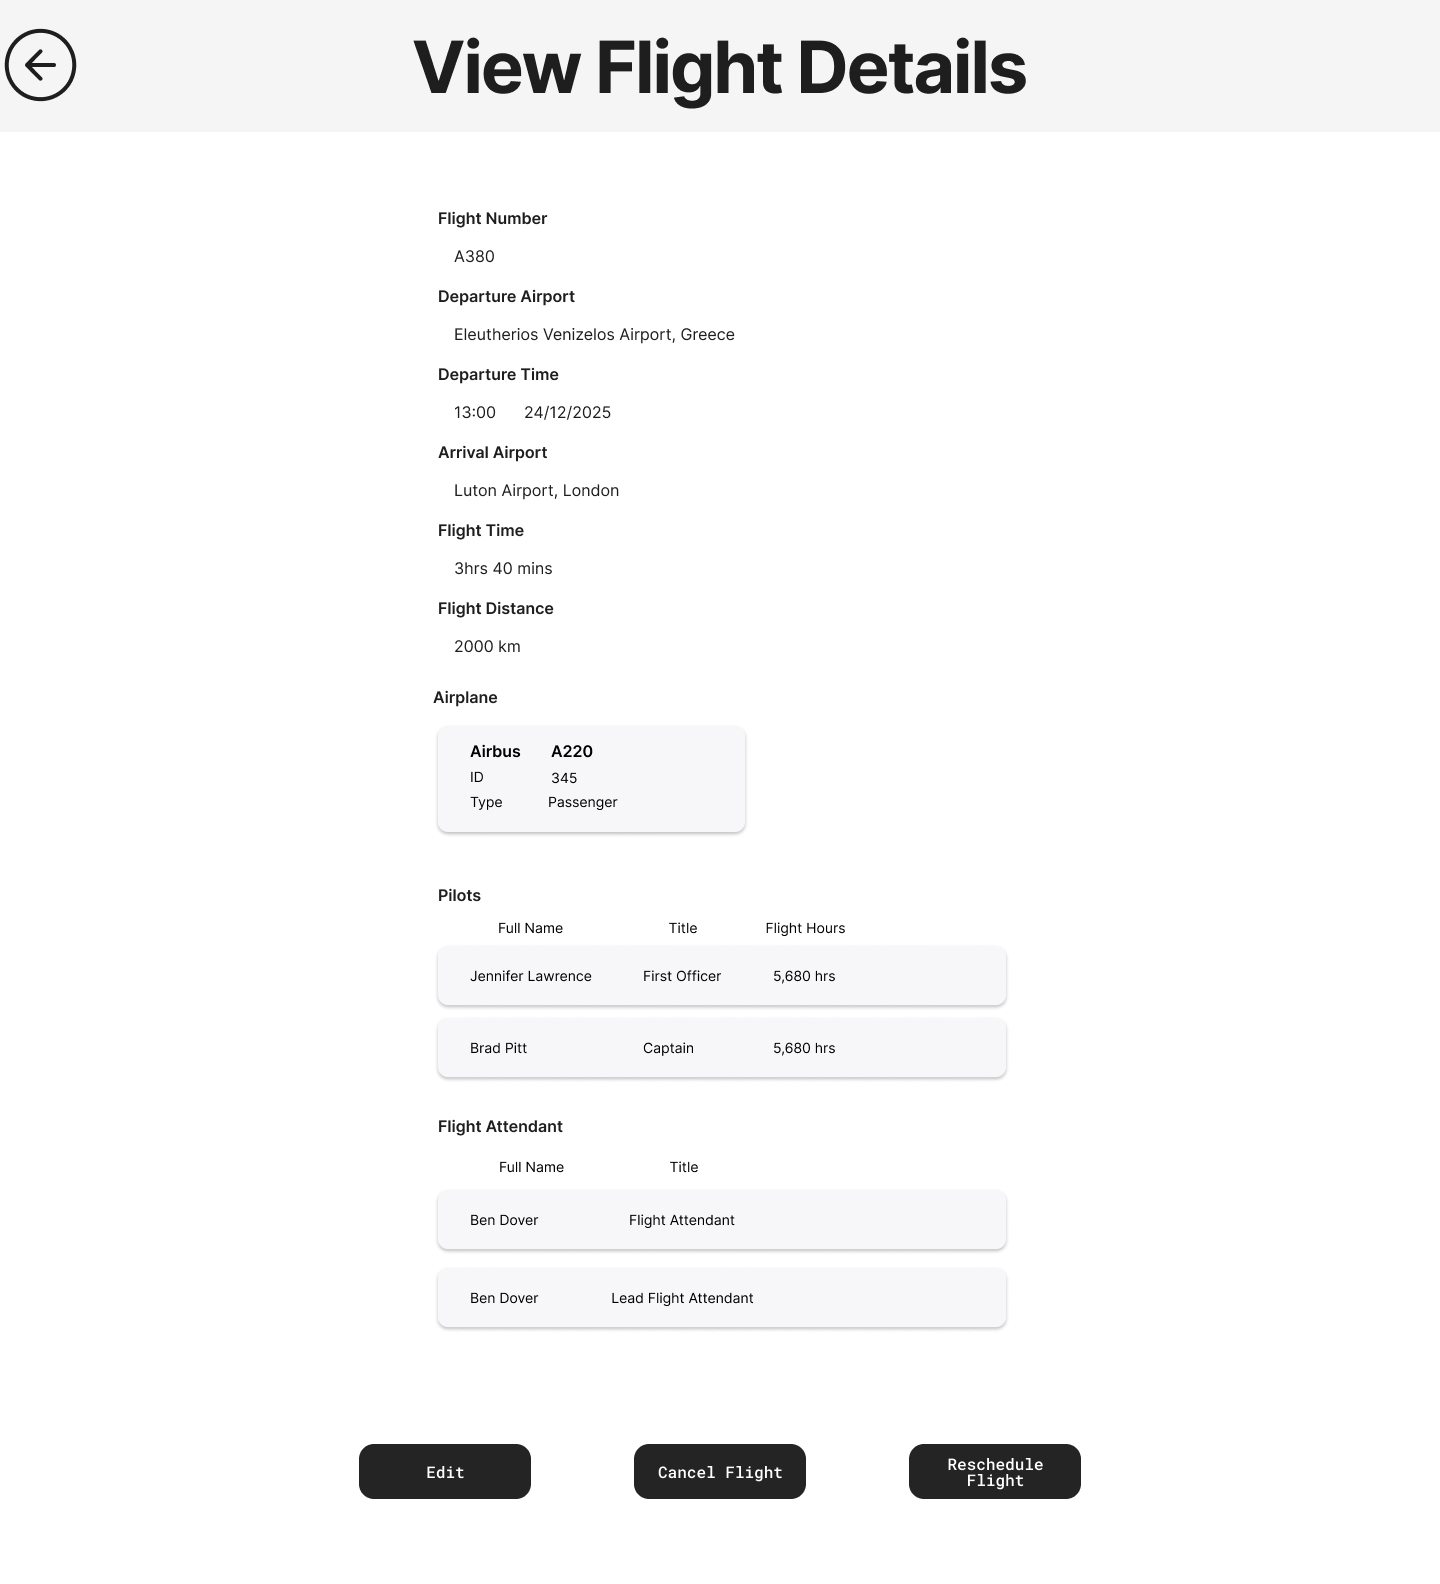
\includegraphics[width=0.75\textwidth]{../mockup-screens/flight-management/Flight-Details.png}
		\caption{Flight Details}
		\label{screen:flight-details}
	\end{figure}

	\begin{figure}[H]
		\centering
		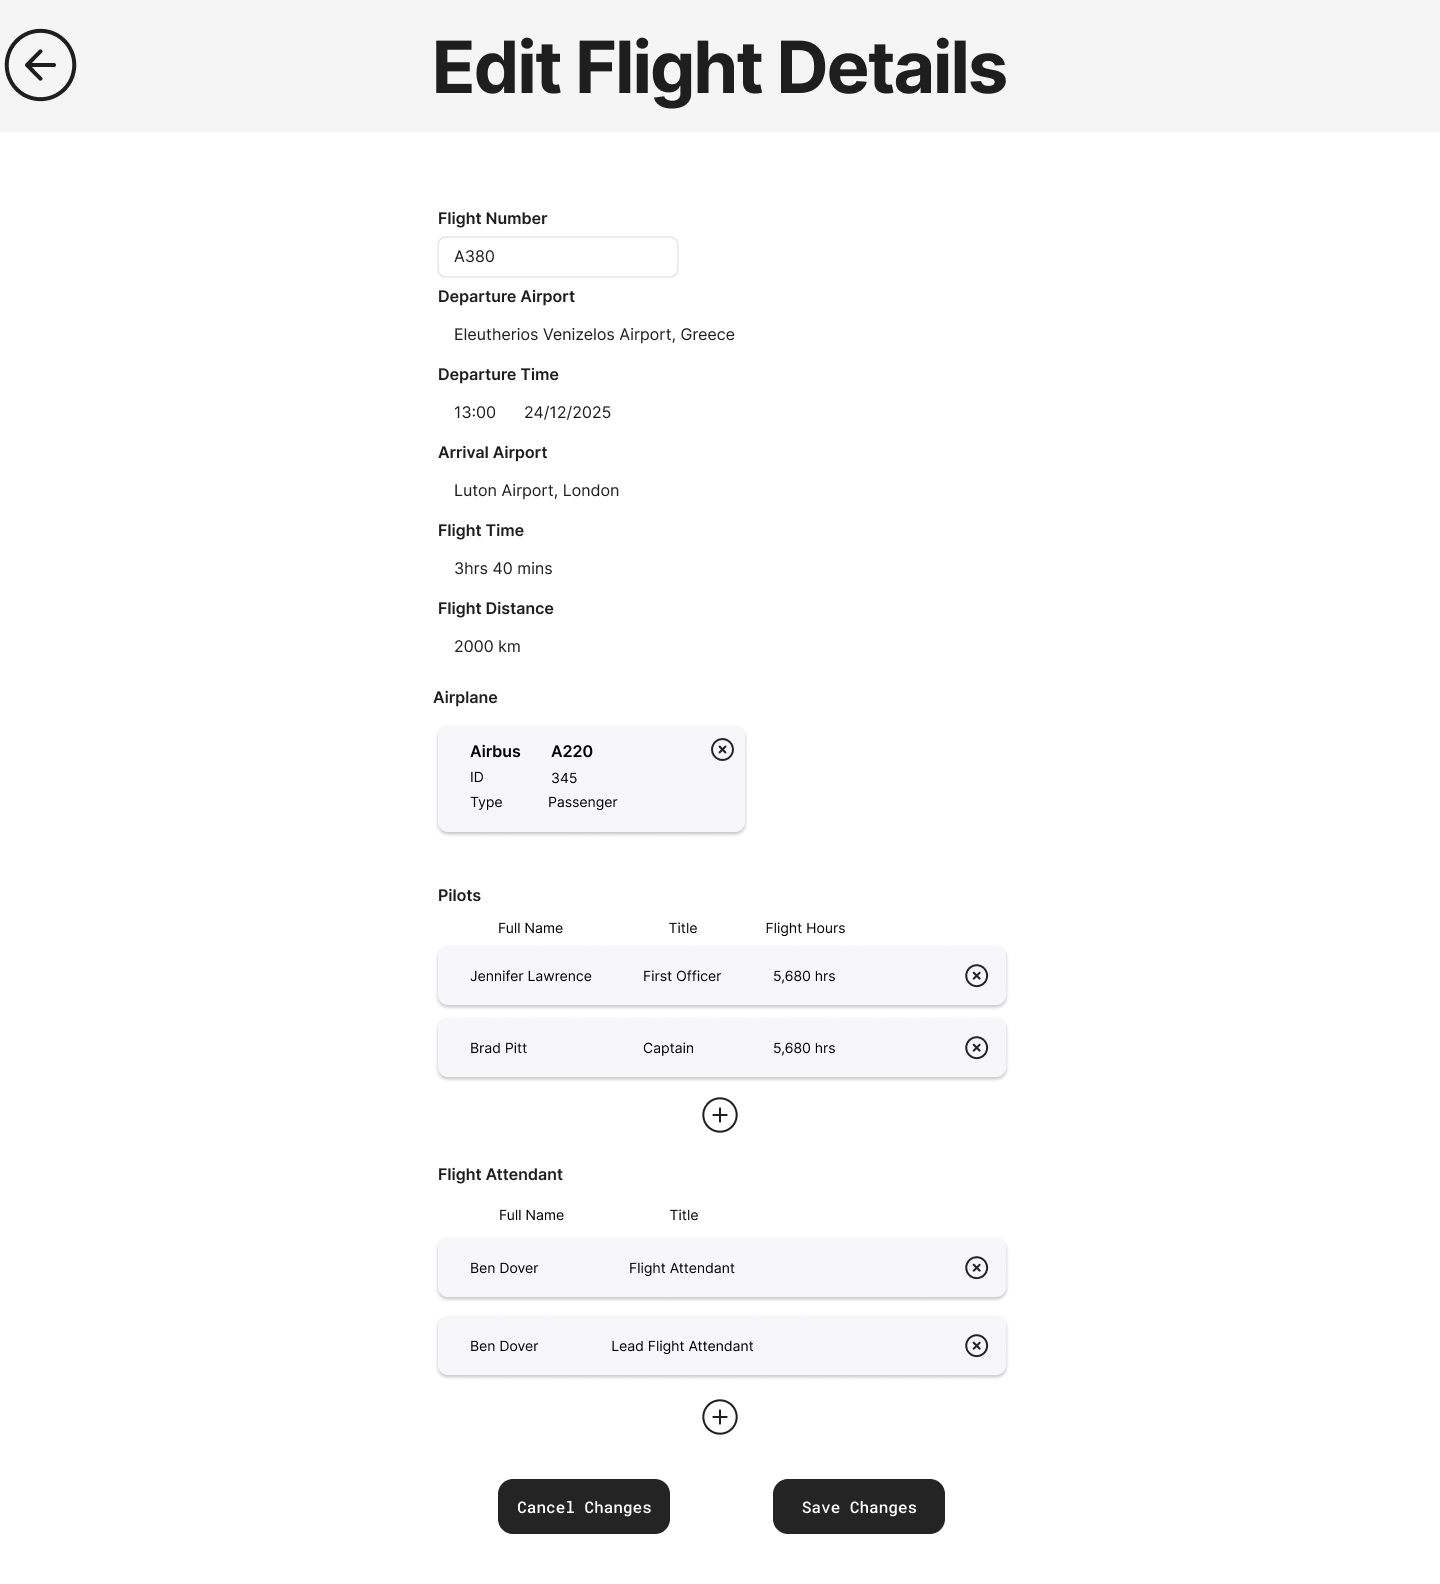
\includegraphics[width=0.5\textwidth]{../mockup-screens/flight-management/Flight-Edit.png}
		\caption{Edit Flight}
		\label{screen:Edit-Flight}
	\end{figure}


	\begin{figure}[H]
		\centering
		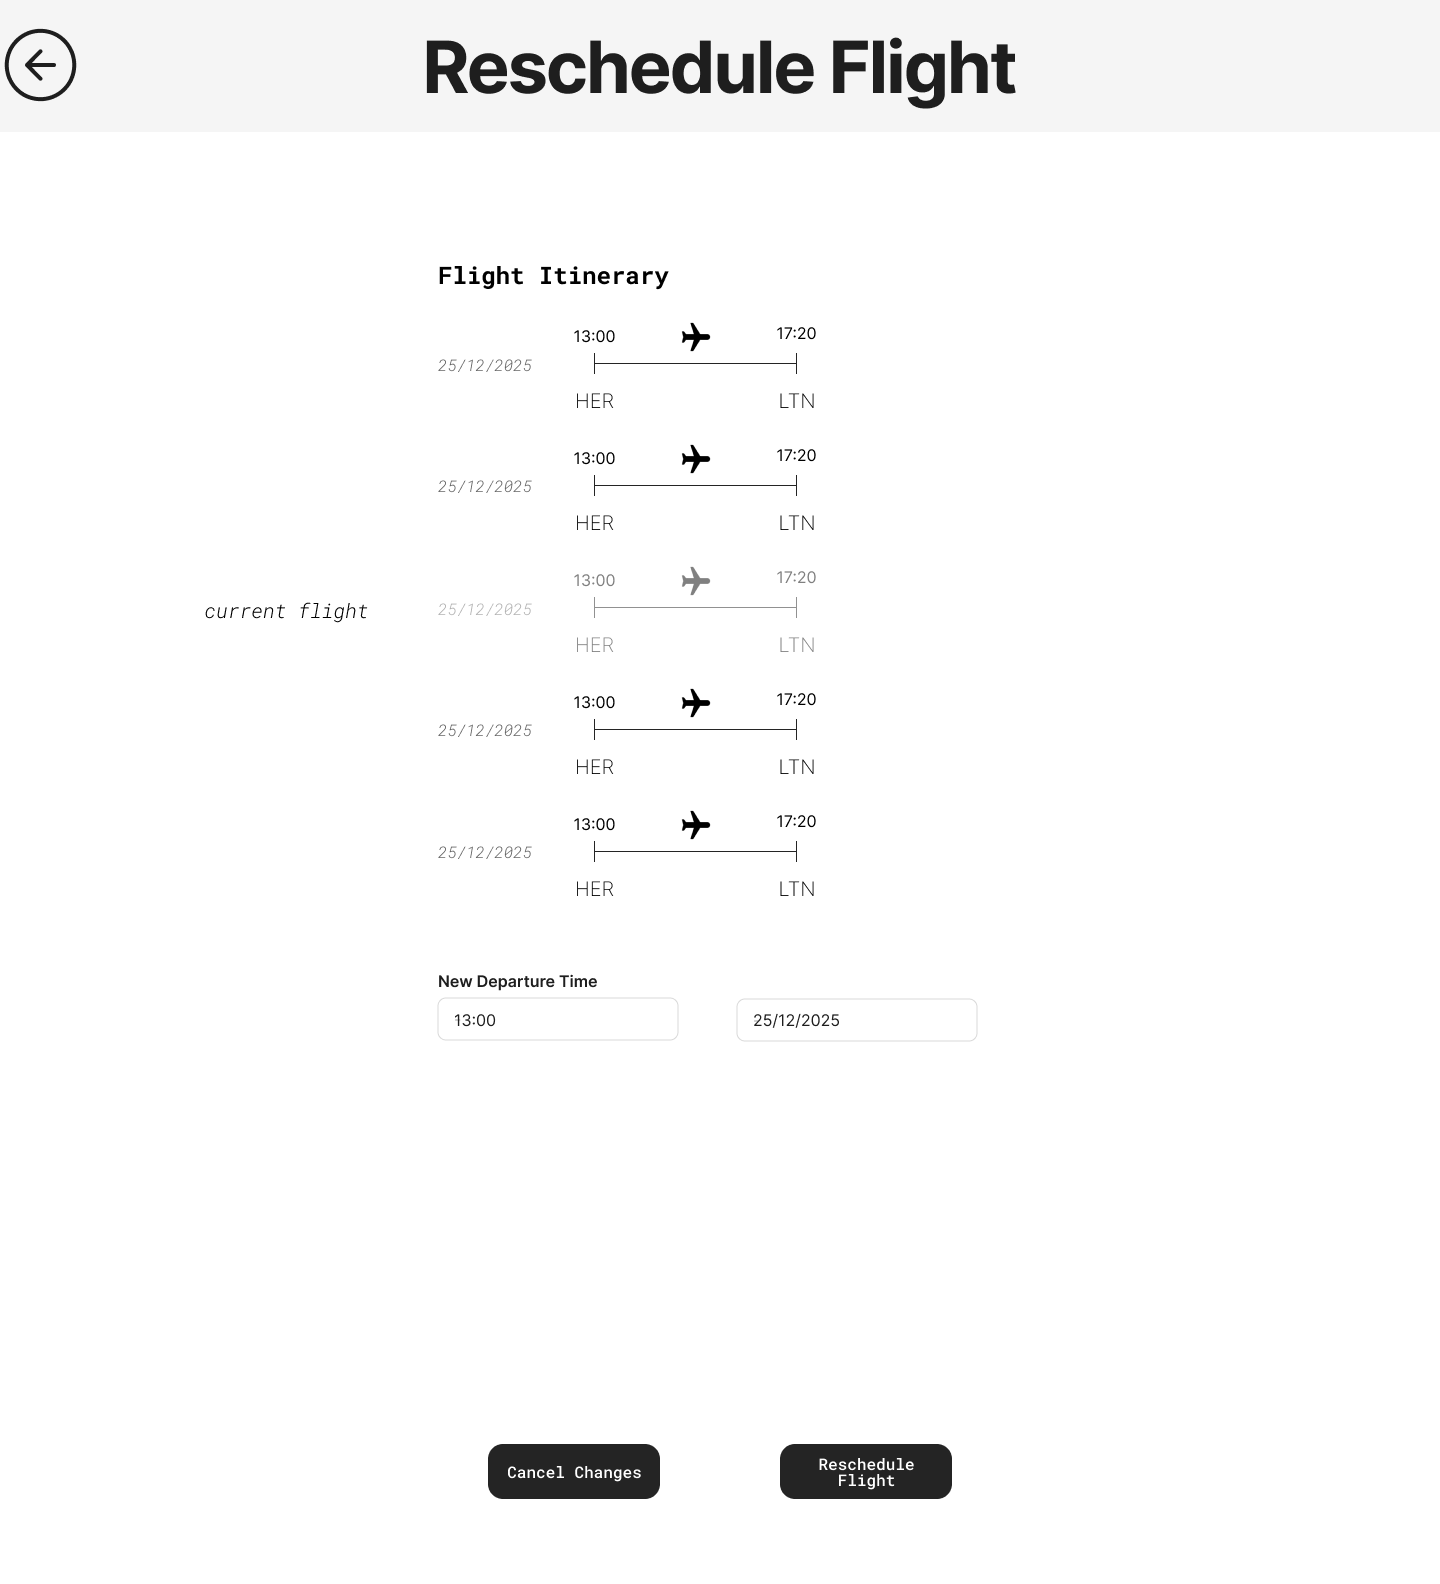
\includegraphics[width=0.5\textwidth]{../mockup-screens/flight-management/Flight-Reschedule.png}
		\caption{Flight Reschedule}
		\label{screen:Flight-Reschedule}
	\end{figure}
	
	\subsection{Διαχείριση Εργαζομένων}
	Το σύστημα προσφέρει τα ακόλουθα εργαλεία για τη διαχείριση των υπαλλήλων των αεροπορικών εταιρειών:
	\begin{enumerate}
		\item Τύποι εργαζομένων και αρμοδιότητες εργασίας: Πληροφορίες για τους πιλότους, τους αεροσυνοδούς, το προσωπικό εδάφους και τους ρόλους τους.
		\item Οι απαιτήσεις σε πλήρωμα καθορίζονται από το σύστημα, το οποίο λαμβάνει υπόψη τις αργίες και τις περιόδους ανάπαυσης κατά τον προσδιορισμό του αριθμού των μελών του πληρώματος που απαιτούνται για κάθε πτήση.
		\item Εύρεση υπαλλήλων από λίστα  : Οι εργαζόμενοι μπορούν να βρεθούν ευκολά από τον διαχειριστή με την χρήση φίλτρων .
	\end{enumerate}
        Στο σχήμα \ref{screen:Employee logs 1} παρουσιάζεται η οθόνη που σου δείχνει όλους τους υπάλληλους που περιέχει το σύστημα.
	Τα φίλτρα του δίνουν την δυνατότητα να βρουν πιο εύκολα ομάδες υπαλλήλων χρησιμοποιώντας ένα ή περισσότερα από τα δοσμένα φίλτρα  . Επίσης του δίνει την δυνατότητα να επιλέξει έναν υπάλληλο. 
	
	Στο σχήμα \ref{screen:Employee logs 2} παρουσιάζει στον διαχειριστή της εταιρίας  όλα τα στοιχεία του υπάλληλου που έχει επιλεχτεί . Ο χρήστης μπορεί να αλλάξει τα στοιχεία του εργαζόμενου καθώς και να ενημερώσει τις ώρες εργασίας και αν είναι ενεργός  .
	\begin{figure}[H]
		\centering
		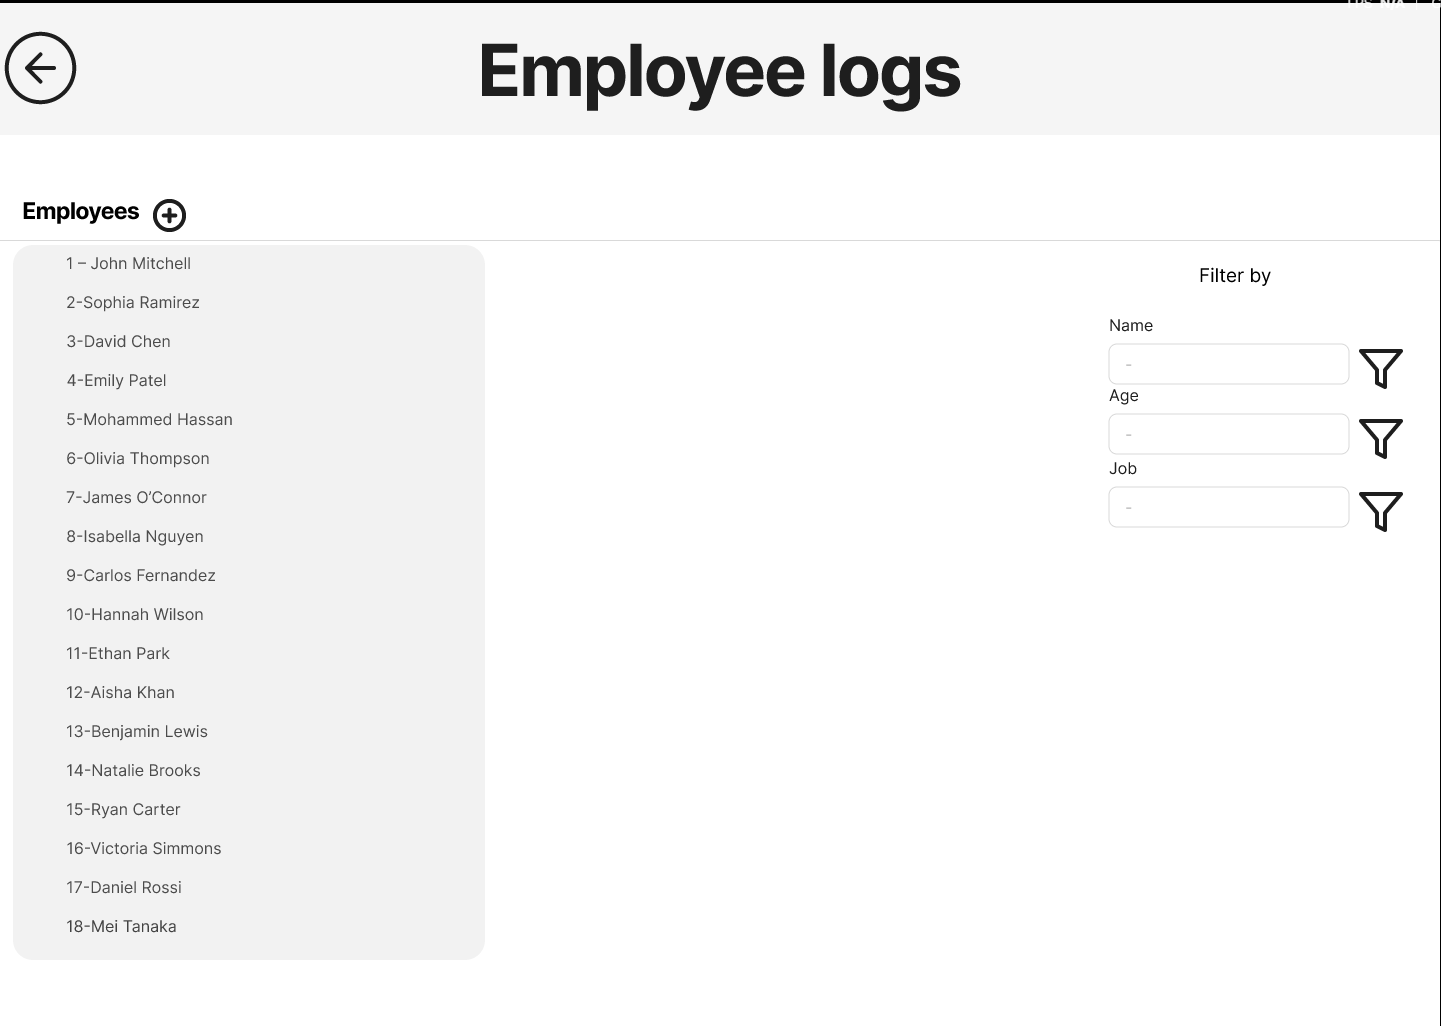
\includegraphics[width=0.5\textwidth]{../mockup-screens/employee logs/Employee logs 1.png}
		\caption{Flight Reschedule}
		\label{screen:Employee logs 1}
	\end{figure}
	
	\begin{figure}[H]
		\centering
		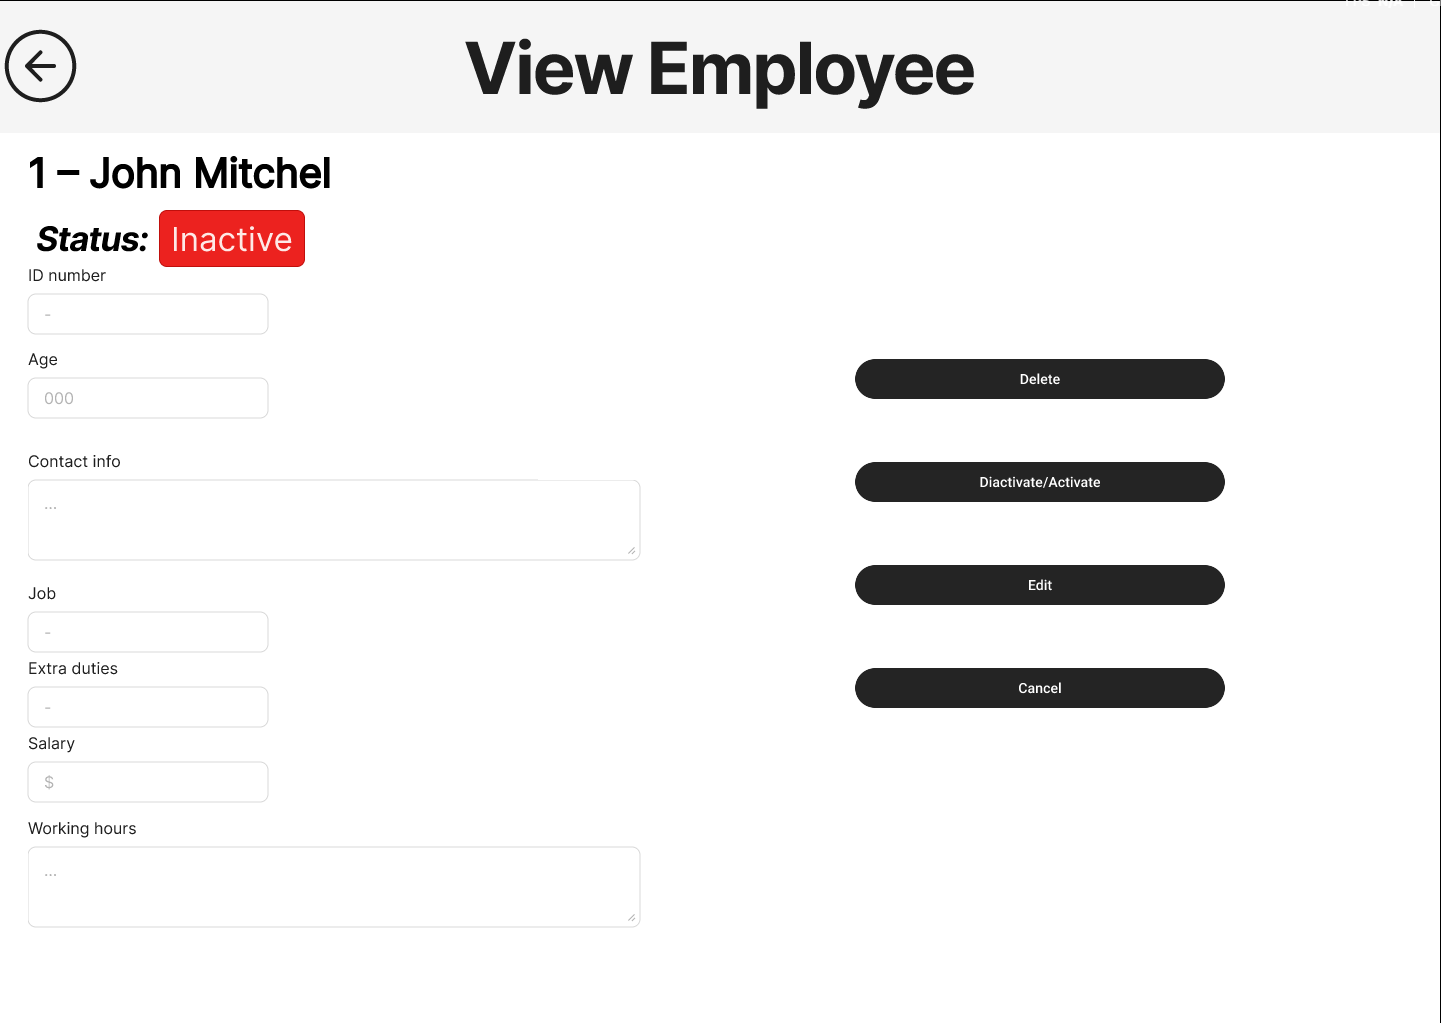
\includegraphics[width=0.5\textwidth]{../mockup-screens/employee logs/Employee logs 2.png}
		\caption{Flight Reschedule}
		\label{screen:Employee logs 2}
	\end{figure}
	
	\subsection{Διαχείριση Αεροδρομίου}
	Το σύστημα διαχειρίζεται δεδομένα που σχετίζονται με το αεροδρόμιο, όπως:
	\begin{enumerate}
		\item Αποθήκευση δεδομένων αεροδρομίου: Η τοποθεσία, η χωρητικότητα , το ωράριο κτλ. όπου διατηρούνται σε αρχείο.
		\item Λίστα όλων διαθέσιμων αεροδρόμιων τις εταιρίας.
		\item Η δυνατότητα να αλλάξει τα στοιχεία του αεροδρομίου καθώς και την κατάσταση λειτουργείας του.
	\end{enumerate}
	
         Στο σχήμα \ref{screen:Airport logs 1} παρουσιάζεται η οθόνη που σου δείχνει όλα τα αεροδρόμια που περιέχει το σύστημα. Ο χρήστης μπορεί να επιλέξει ένα από τα αεροδρόμια 
	Στο σχήμα \ref{screen:Airport logs 2} παρουσιάζει στον διαχειριστή της εταιρίας  όλα τα στοιχεία του αεροδρομίου που έχει επιλεχτεί . Ο χρήστης μπορεί να αλλάξει τα στοιχεία του αεροδρομίου καθώς και την κατάσταση λειτουργίας. 
	\begin{figure}[H]
		\centering
		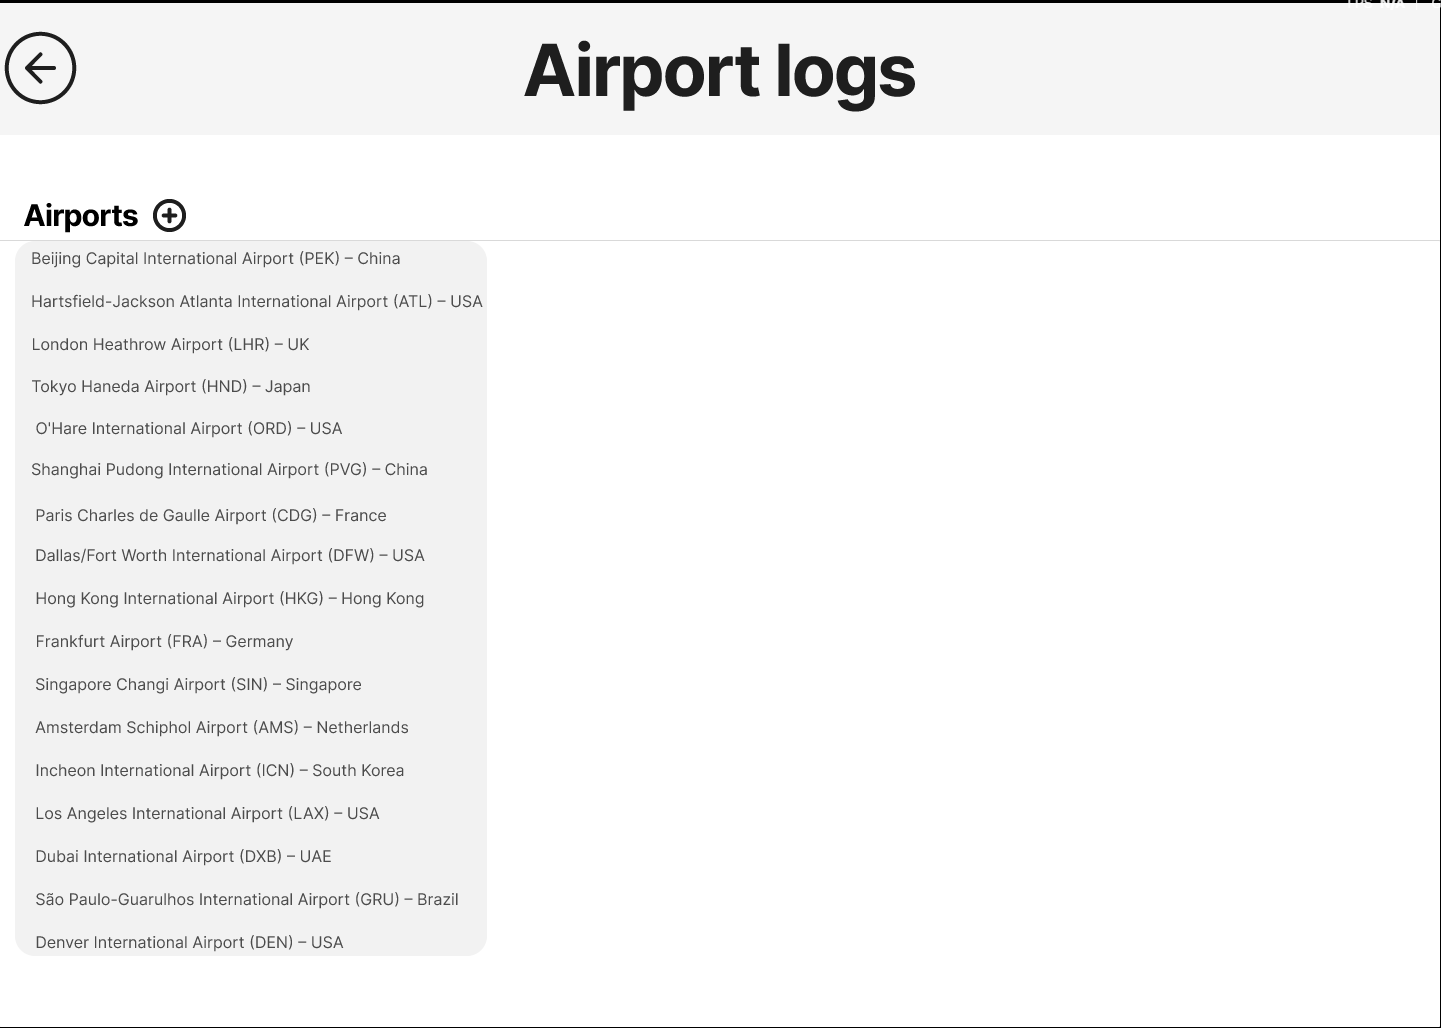
\includegraphics[width=0.5\textwidth]{../mockup-screens/airport logs/Airport logs 1.png}
		\caption{Flight Reschedule}
		\label{screen:Airport logs 1}
	\end{figure}

	\begin{figure}[H]
		\centering
		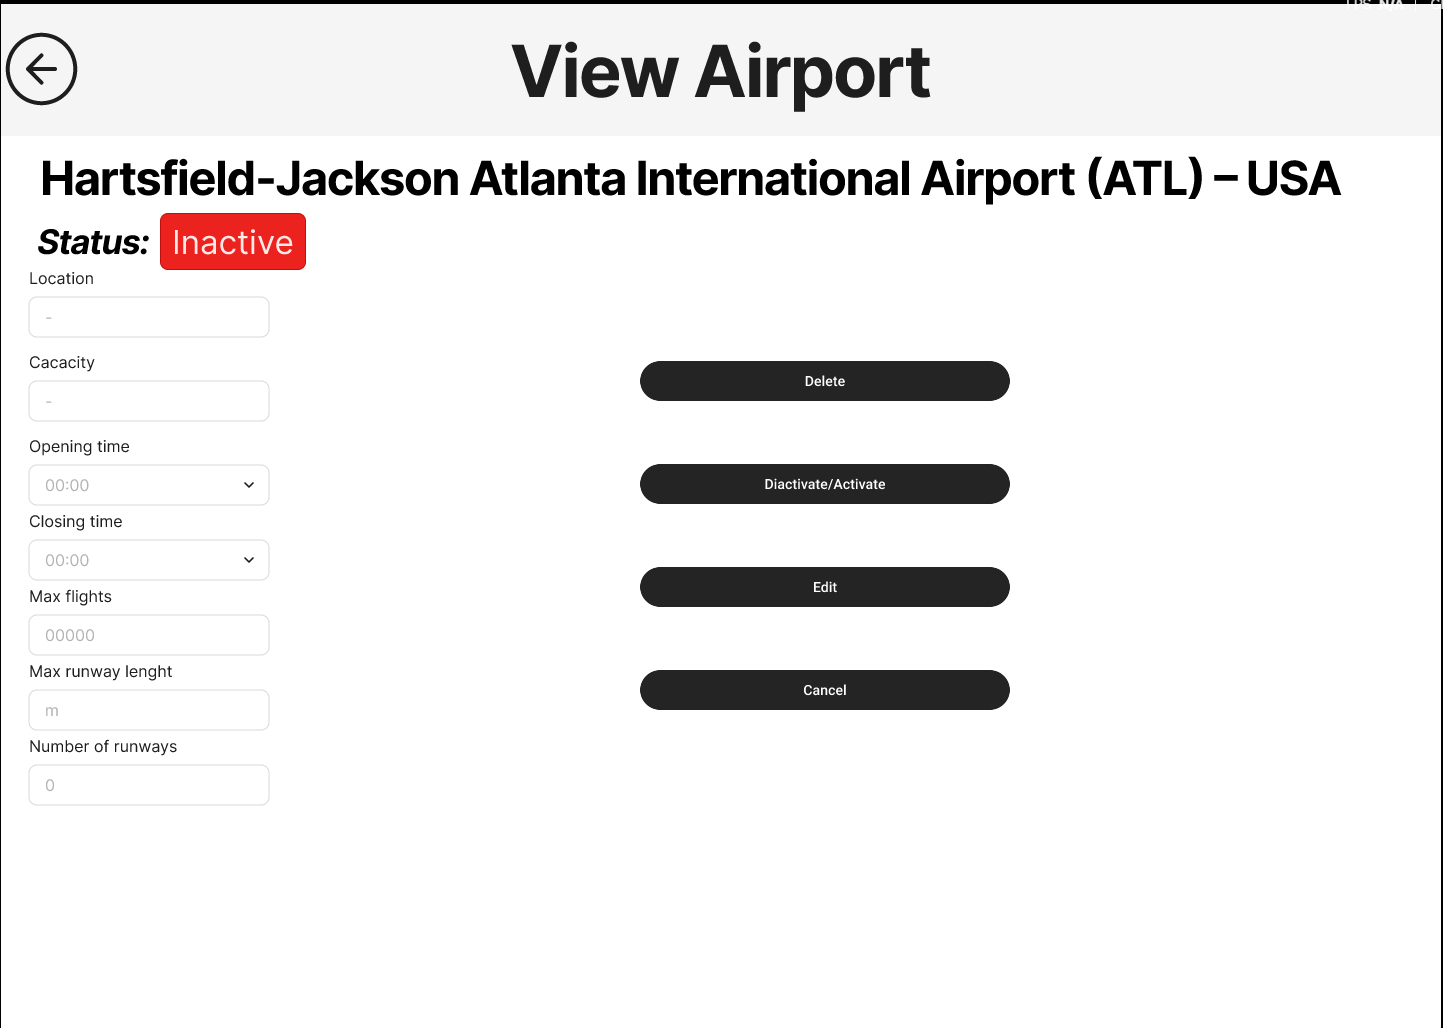
\includegraphics[width=0.5\textwidth]{../mockup-screens/airport logs/Airport logs 2.png}
		\caption{Flight Reschedule}
		\label{screen:Airport logs 2}
	\end{figure}

\subsection{Διαχείριση Αεροπλανων}
	Το σύστημα προσφέρει τα ακόλουθα εργαλεία για τη διαχείριση των αεροπλανων των αεροπορικών εταιρειών:
	\begin{enumerate}
		\item Τύποι αεροπλάνων και τα στοιχεία τους: Πληροφορίες για τα αεροπλάνα, τις δυνατότητες τους και τις προδιαγραφες τους .
		\item Η δυνατοτητα να αλλαξει τα στοιχεια του αεροπανου καθως και την κατασταση λειτουργιας του.
		\item Εύρεση αεροπλάνων από λίστα  : Τα αεροπλάνα μπορούν να βρεθούν ευκολά από τον διαχειριστή με την χρήση φίλτρων .
	\end{enumerate}
        Στο σχήμα \ref{screen:Airplane_logs_1} παρουσιάζεται η οθόνη που σου δείχνει όλους τα αεροπλάνα που περιέχει το σύστημα.
	Τα φίλτρα του δίνουν την δυνατότητα να βρουν πιο εύκολα ομάδες αεροπλάνων χρησιμοποιώντας ένα ή περισσότερα από τα δοσμένα φίλτρα  . Επίσης του δίνει την δυνατότητα να επιλέξει ένα αεροπλάνο. 
	
	Στο σχήμα \ref{screen:Airplane_logs_2} παρουσιάζει στον διαχειριστή της εταιρίας  όλα τα στοιχεία του αεροπλανου που έχει επιλεχτεί . Ο χρήστης μπορεί να αλλάξει τα στοιχεία του αεροπλάνου καθώς και να ενημερώσει την κατάσταση λειτουργείας του .

	\begin{figure}[H]
		\centering
		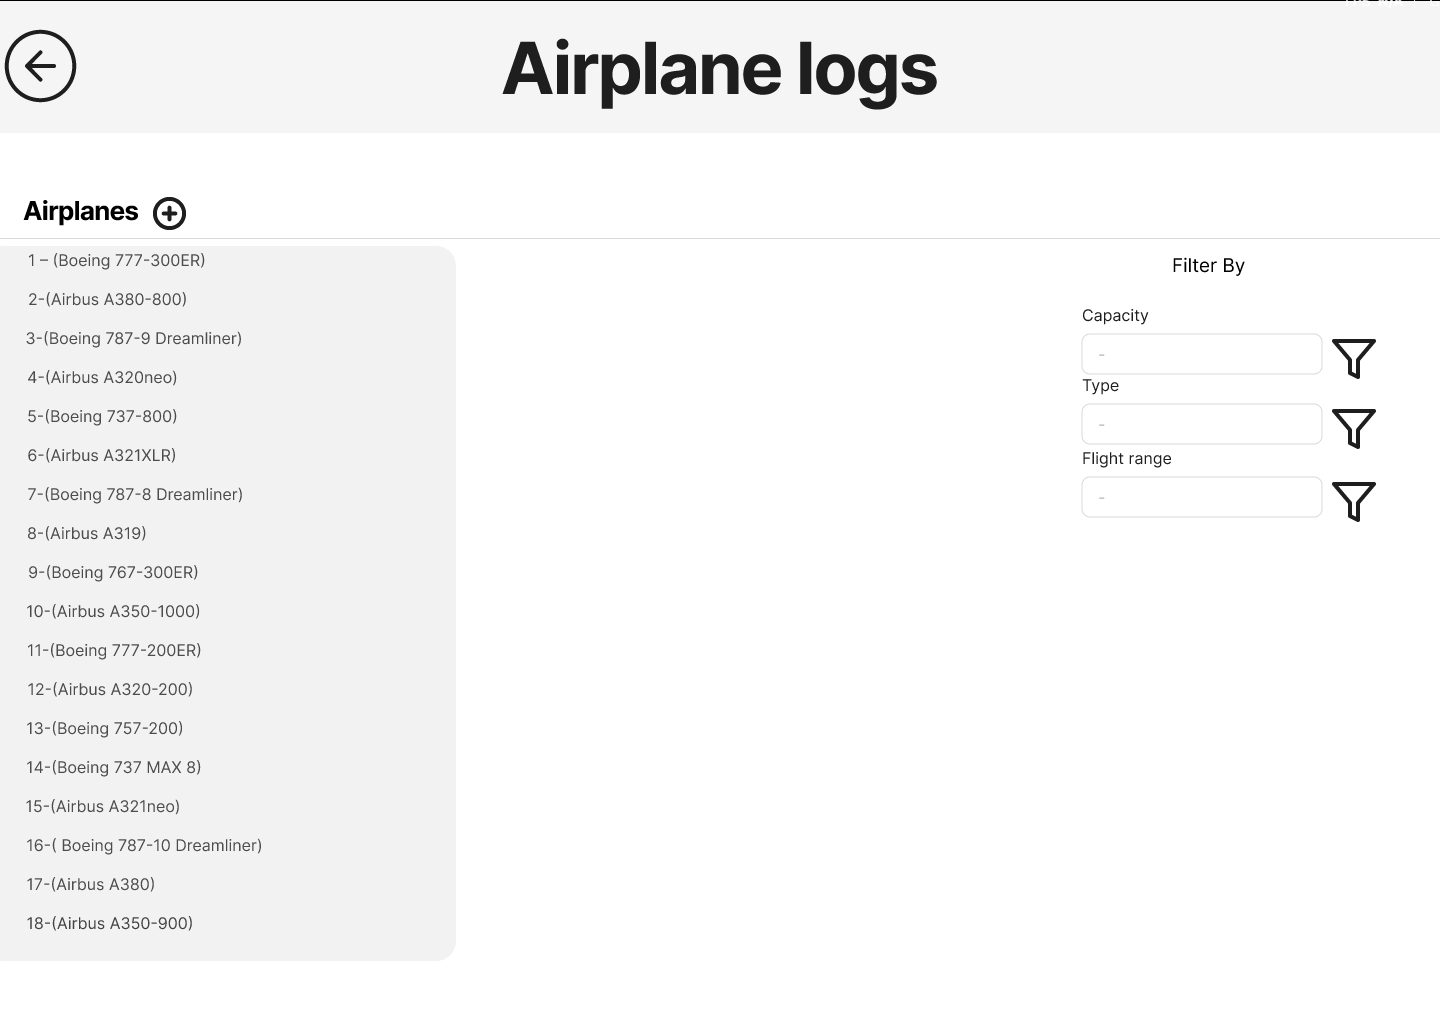
\includegraphics[width=0.5\textwidth]{../mockup-screens/airplane logs/Airplane_logs_1.png}
		\caption{Flight Reschedule}
		\label{screen:Airplane_logs_1}
	\end{figure}

	\begin{figure}[H]
		\centering
		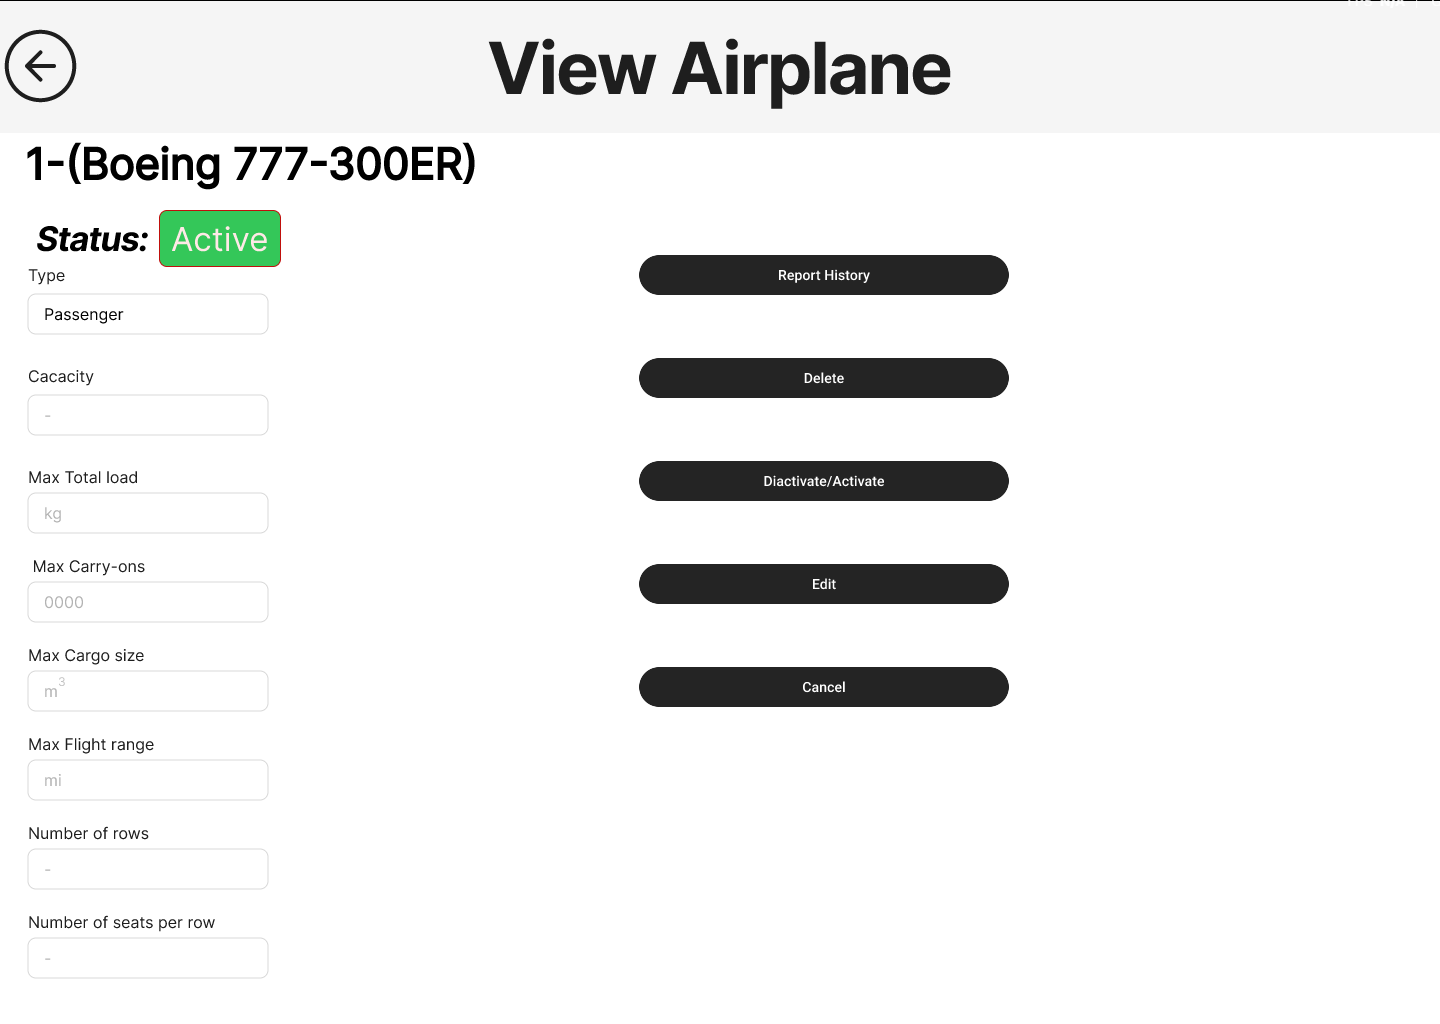
\includegraphics[width=0.5\textwidth]{../mockup-screens/airplane logs/Airplane_logs_2.png}
		\caption{Flight Reschedule}
		\label{screen:Airplane_logs_2}
	\end{figure}


	\subsection{Αναφορές}
	Το σύστημα αποθηκεύει και διαχειρίζεται αναφορές από τους πιλότους για τις πτήσεις με τον εξής τρόπο:
	\begin{enumerate}
		\item Δυνατότητα αυτόματης ακύρωσης πτήσεων αν κριθεί από το σύστημα ότι είναι απαραίτητη η συντήρησή του
        \item Δυνατότητα χειροκίνητης ανάγνωσης των αναφορών από τους διαχειριστές και ακύρωση των μελλοντικών πτήσεων αν κριθεί απαραίτητο για συντήρηση. 
	\end{enumerate}

    Στο σχήμα \ref{fig:pilot_reports_1} ο χρήστης βλέπει μια λίστα με όλα τα διαθέσιμα αεροπλάνα και έχει την δυνατότητα να επιλέξει ένα

    Στο σχήμα \ref{fig:Pilot_reports_2} ο χρήστης βλέπει μια λίστα με τις πτήσεις που έχουν εκτελεστεί με το αεροπλάνο που επέλεξε στην προηγούμενη οθόνη και επιλέγει μία

    Στο σχήμα \ref{fig:Pilot_reports_3} Ο χρήστης βλέπει την αναφορά των πιλότων που γράφτηκε για αυτή την πτήση και έχει την επιλογή να στείλει το αεροσκάφος για συντήρηση.
    \begin{figure}[H]
        \centering
        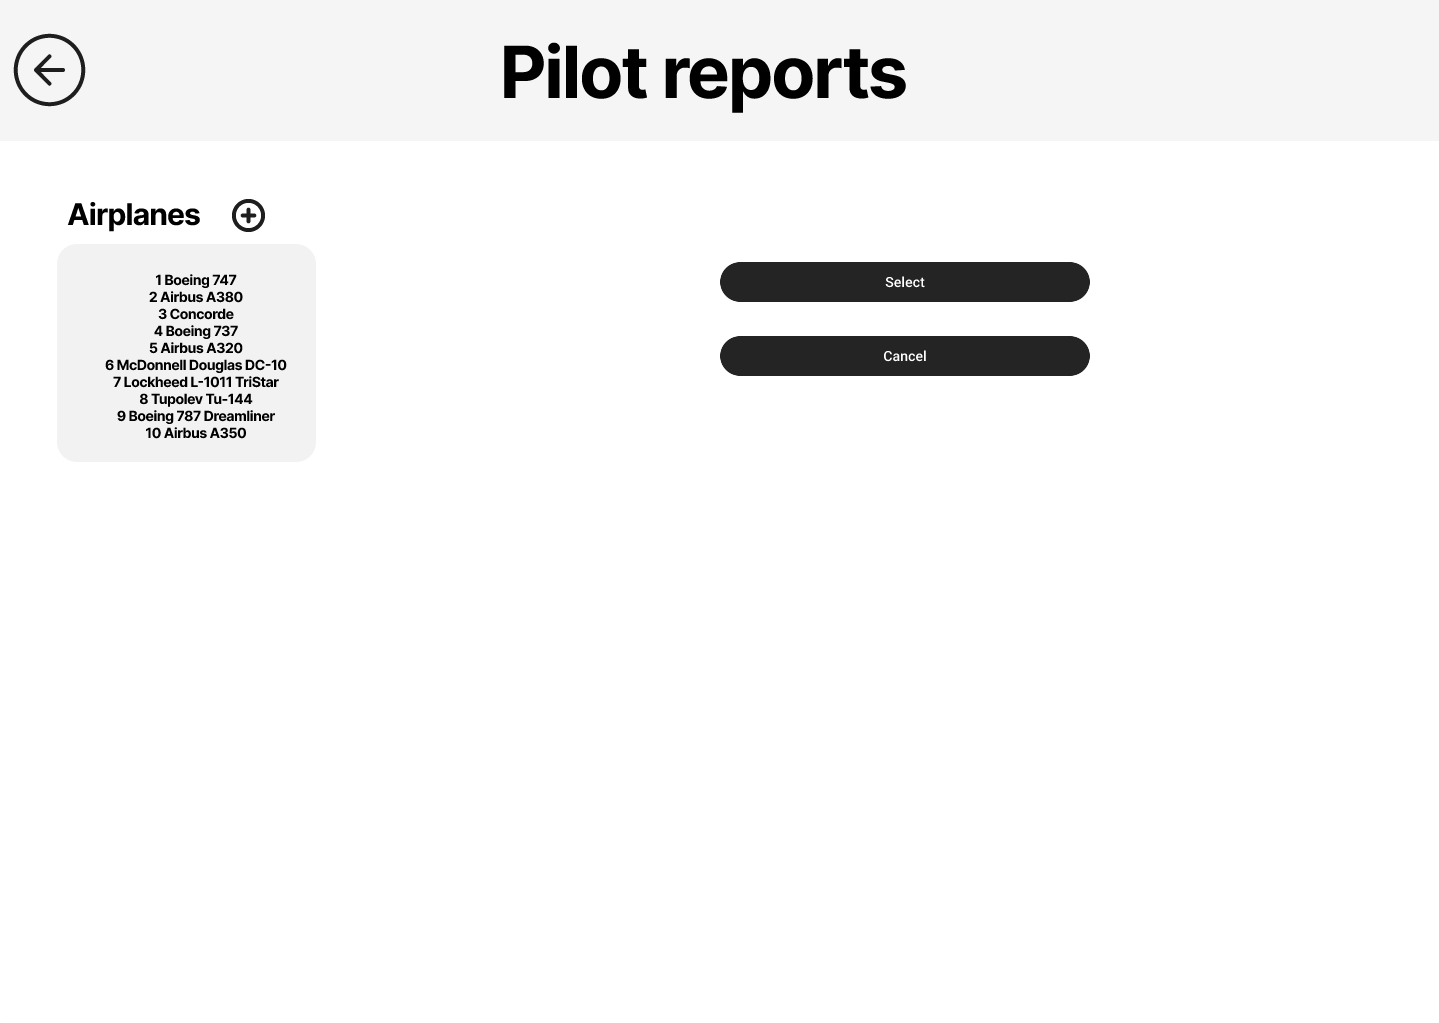
\includegraphics[width=0.75\linewidth]{../mockup-screens/pilot reports mockups/Pilot_reports_1.png}
        \caption{Choose plane}
        \label{fig:pilot_reports_1}
    \end{figure}
    
    \begin{figure}[H]
        \centering
        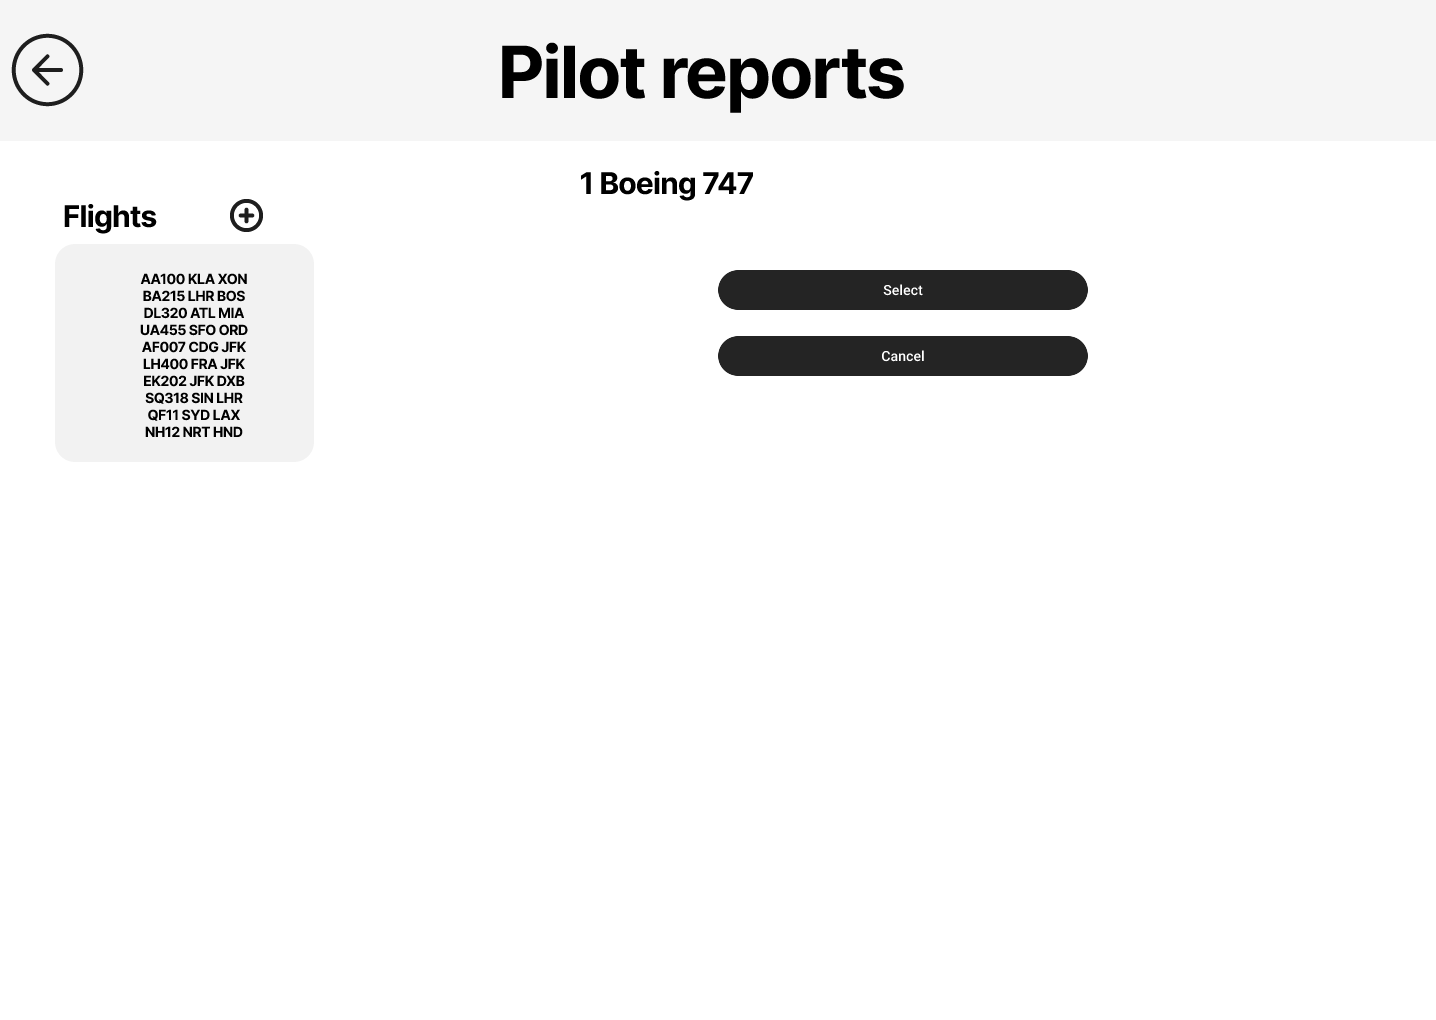
\includegraphics[width=0.75\linewidth]{../mockup-screens/pilot reports mockups/Pilot_reports_2.png}
        \caption{Choose flight}
        \label{fig:Pilot_reports_2}
    \end{figure}

    \begin{figure}[H]
        \centering
        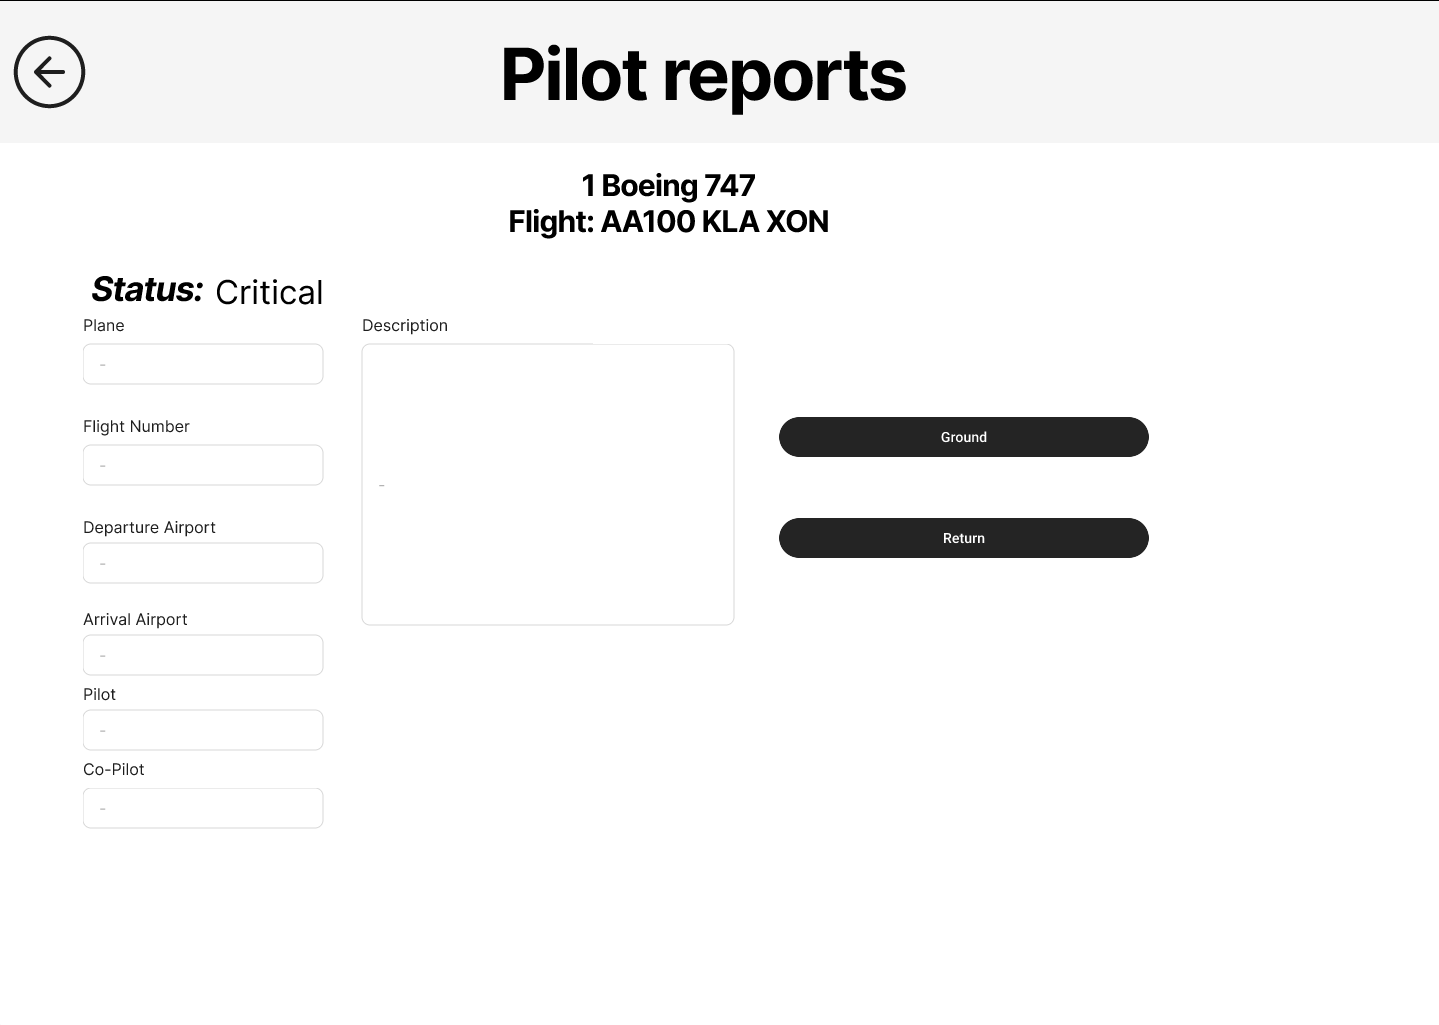
\includegraphics[width=0.75\linewidth]{../mockup-screens/pilot reports mockups/Pilot_reports_3.png}
        \caption{Report}
        \label{fig:Pilot_reports_3}
    \end{figure}
    
	
	\subsection{Διαχείριση Φαγητού και Μενού}
	Το σύστημα διαχειρίζεται επιλογές φαγητού για διαφορετικούς τύπους πτήσεων, όπως:
	\begin{enumerate}
		\item Δημιουργία και αποθήκευση επιλογών μενού φαγητού: Αποθηκεύονται λεπτομέρειες σχετικά με τις επιλογές φαγητού για διαφορετικούς τύπους αεροπλάνων και διάρκειες πτήσεων.
		\item Καθορισμός τιμών τροφίμων: Οι τιμές για κάθε menu  καθορίζονται με βάση το κόστος των τροφίμων που περιέχει.
	\end{enumerate}
    Στο σχήμα \ref{fig:Insert_menu_item} Ο χρήστης εισάγει στα πεδία τα στοιχεία του αντικειμένου που θέλει

    Στο σχήμα \ref{fig:Create_menu} Ο χρήστης βλέπει μια λίστα με όλα τα διαθέσιμα αντικείμενα και επιλέγει κάθε φορά ένα για αν εισάγει στο μενού
    \begin{figure}
        \centering
        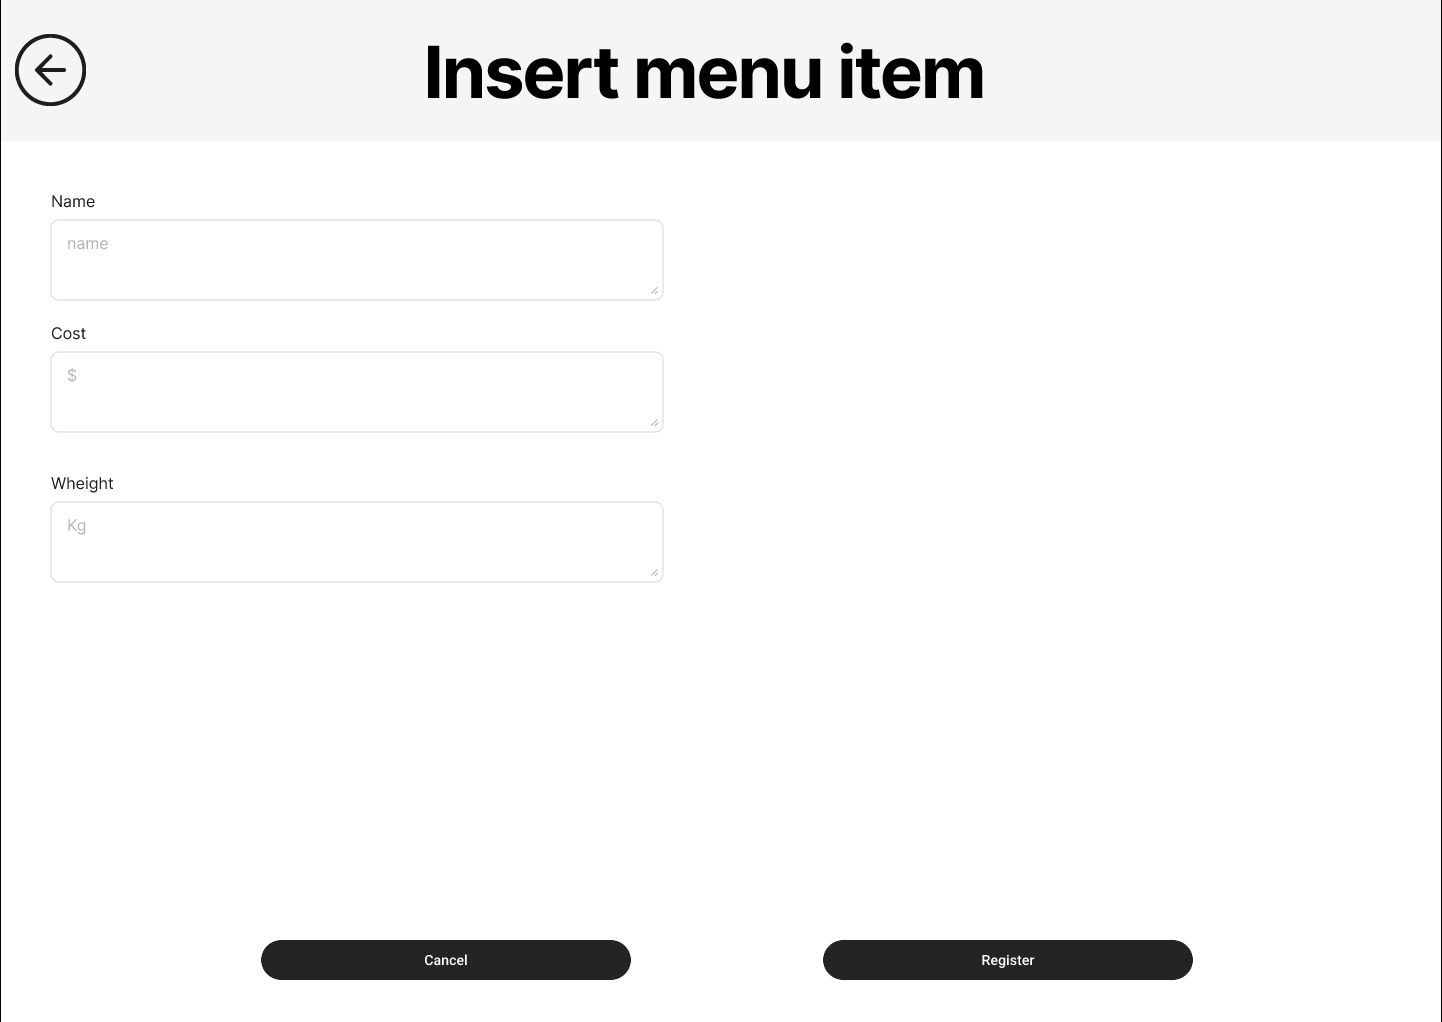
\includegraphics[width=0.75\linewidth]{../mockup-screens/menu case mockups/Insert_menu_item.png}
        \caption{Insert menu item}
        \label{fig:Insert_menu_item}
    \end{figure}

    \begin{figure}
        \centering
        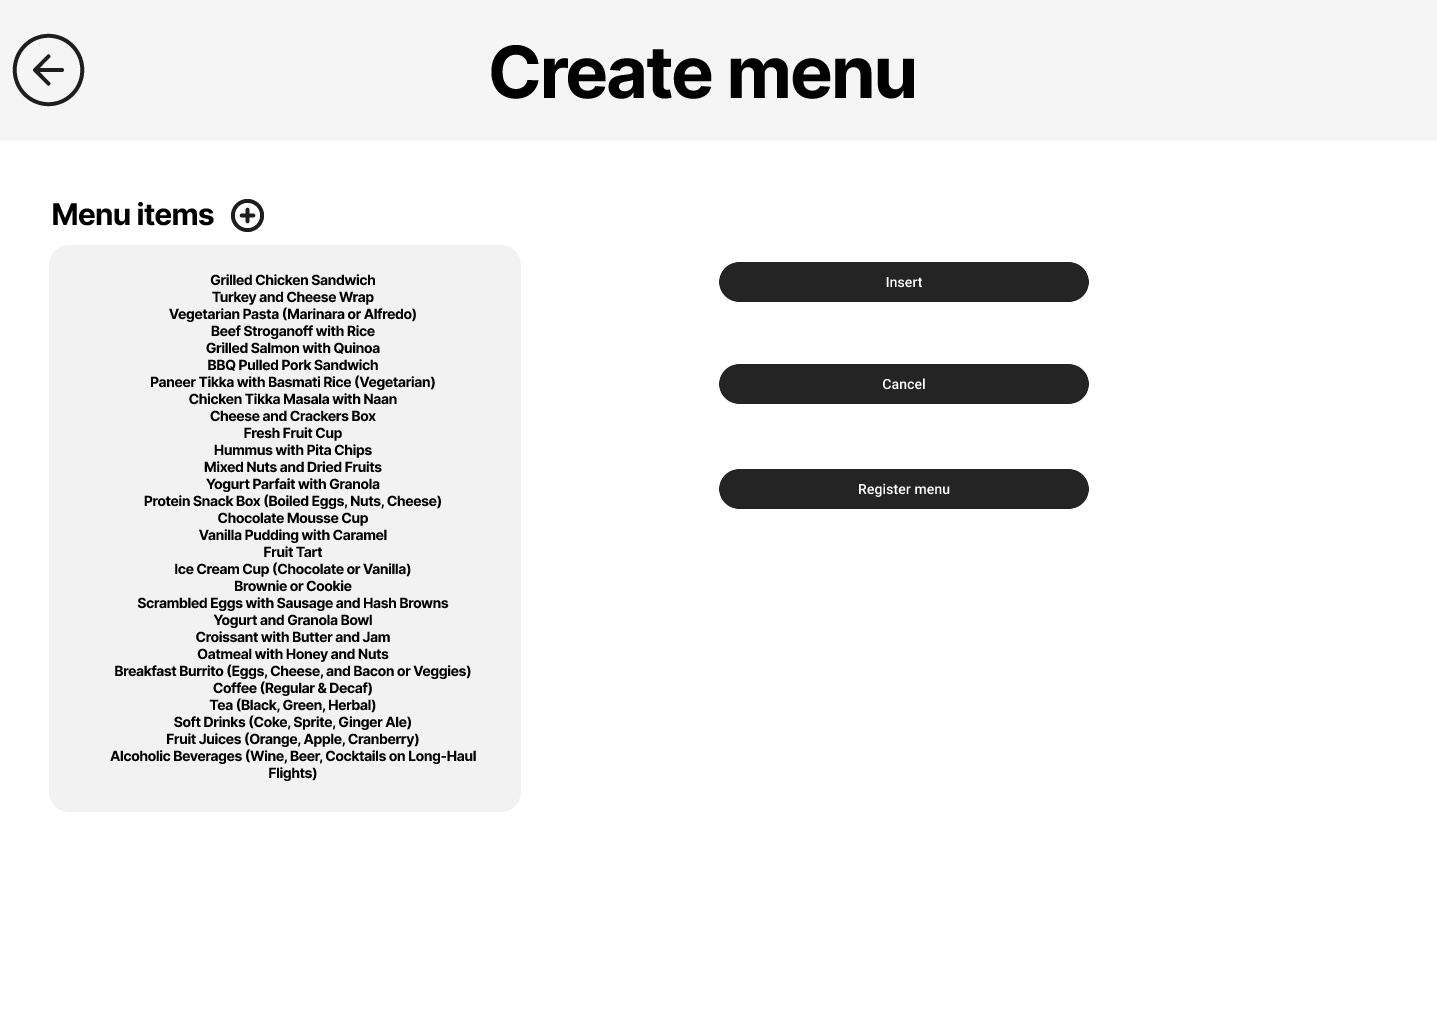
\includegraphics[width=0.75\linewidth]{../mockup-screens/menu case mockups/Create_menu.png}
        \caption{Create menu}
        \label{fig:Create_menu}
    \end{figure}
	\subsection{Ανάθεση Βάρδιας Εργαζομένων}
	\begin{enumerate}
		\item Το σύστημα αντιστοιχίζει εργαζόμενους σε πτήσεις σύμφωνα με προσόντα, διαθεσιμότητα και κανονισμούς ανάπαυσης.
		\item Προγραμματίζει βάρδιες και ειδοποιεί τους υπαλλήλους.
	\end{enumerate}
	
	\subsection{Διαχείριση Εργολάβων}
	Το σύστημα δίνει την δυνατότητα στον διαχειριστή να αποθηκεύει την συνεργασία του με εξωτερικούς συνεργάτες ως εξής:
	\begin{enumerate}
		\item αποθηκεύει και βλέπει όλες τις ενεργές συνεργασίες
		\item έχει την δυνατότητα να ενημερλωσει το σύστημα μετά την ολοκλήρωση μιας εργασίας  
	\end{enumerate}

 	Στο σχήμα \ref{fig:contractor-selection} εμφανίζονται τα πεδία εισαγωγής των στοιχείων της εργασίας όπως όνομα, τύπος, αεροδρόμιο, ημερομηνία και μαι σύντομη περιγραφή

	Στο σχήμα \ref{fig:contractor-assignment} παρουσιάζεται η λίστα με όλες τις εργασίες και μπορεί ο χρήστης με φίλτρα να επιλέξει να δεί μόνο αυτές που τον ενδιαφέρουν όπως πληρωμένες, ενεργές κλπ

	Στο σχήμα \ref{fig:contractor-assignment-form} παρουσιάζονται οι πληροφορίες για την εργασία που έχει επιλέξει ο χρήστης και έχει την δυνατότητα να επιλέξει την ολοκλήρωσή της
 	

    \begin{figure}[H]
        \centering
        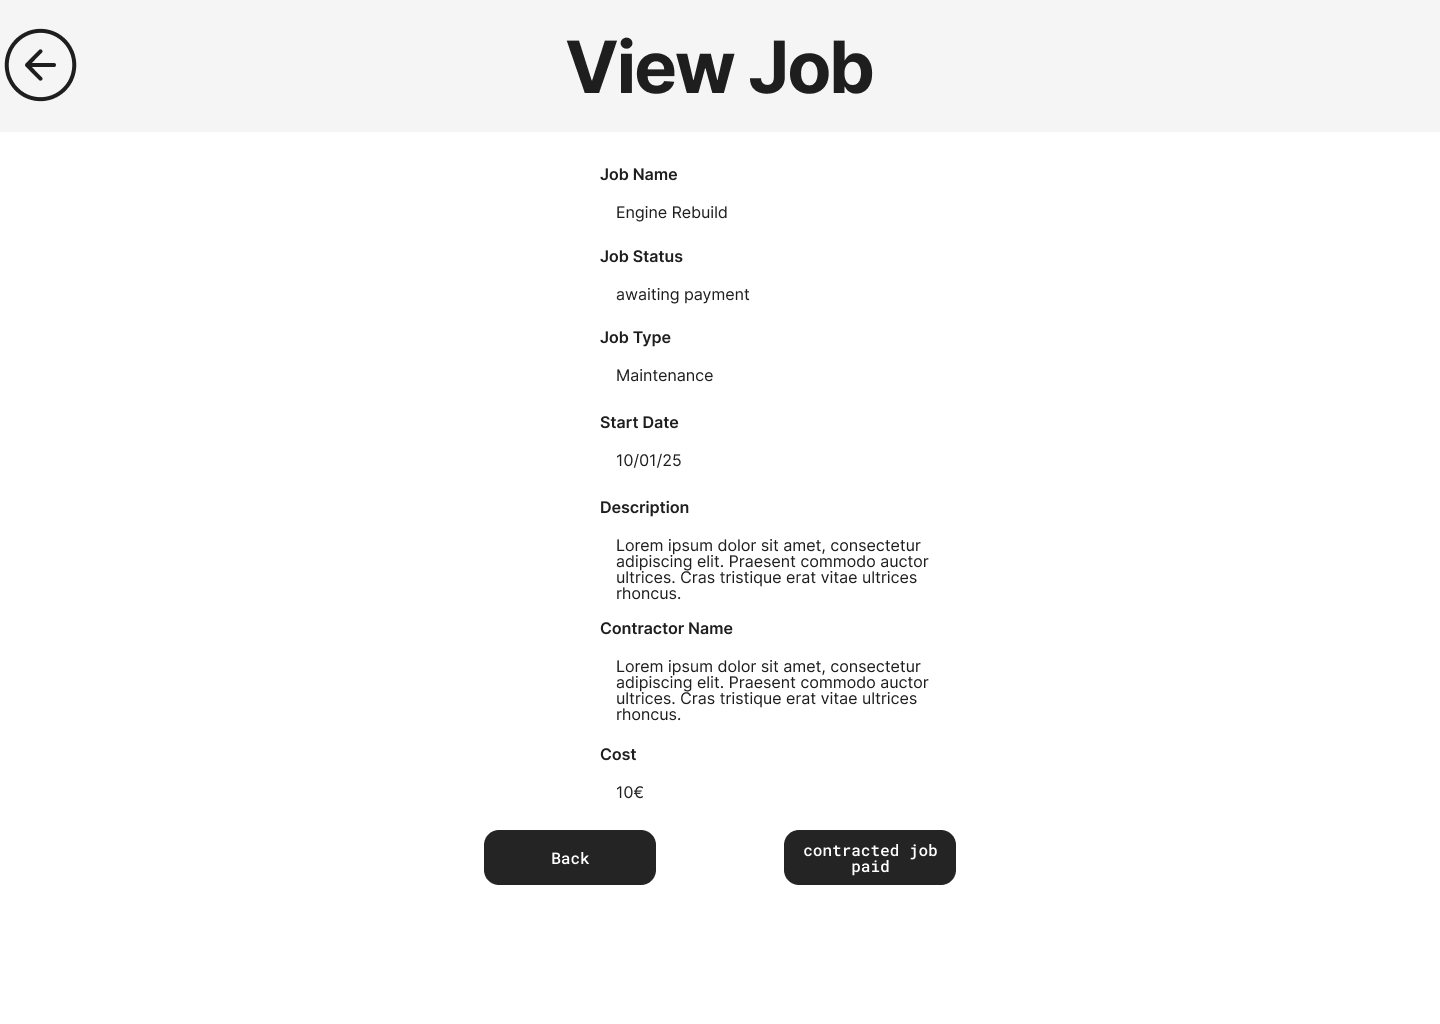
\includegraphics[width=0.75\linewidth]{../mockup-screens/Contractor-mockups/view job.png}
        \caption{Create menu}
        \label{fig:contractor-assignment}
    \end{figure}	

    \begin{figure}[H]
        \centering
        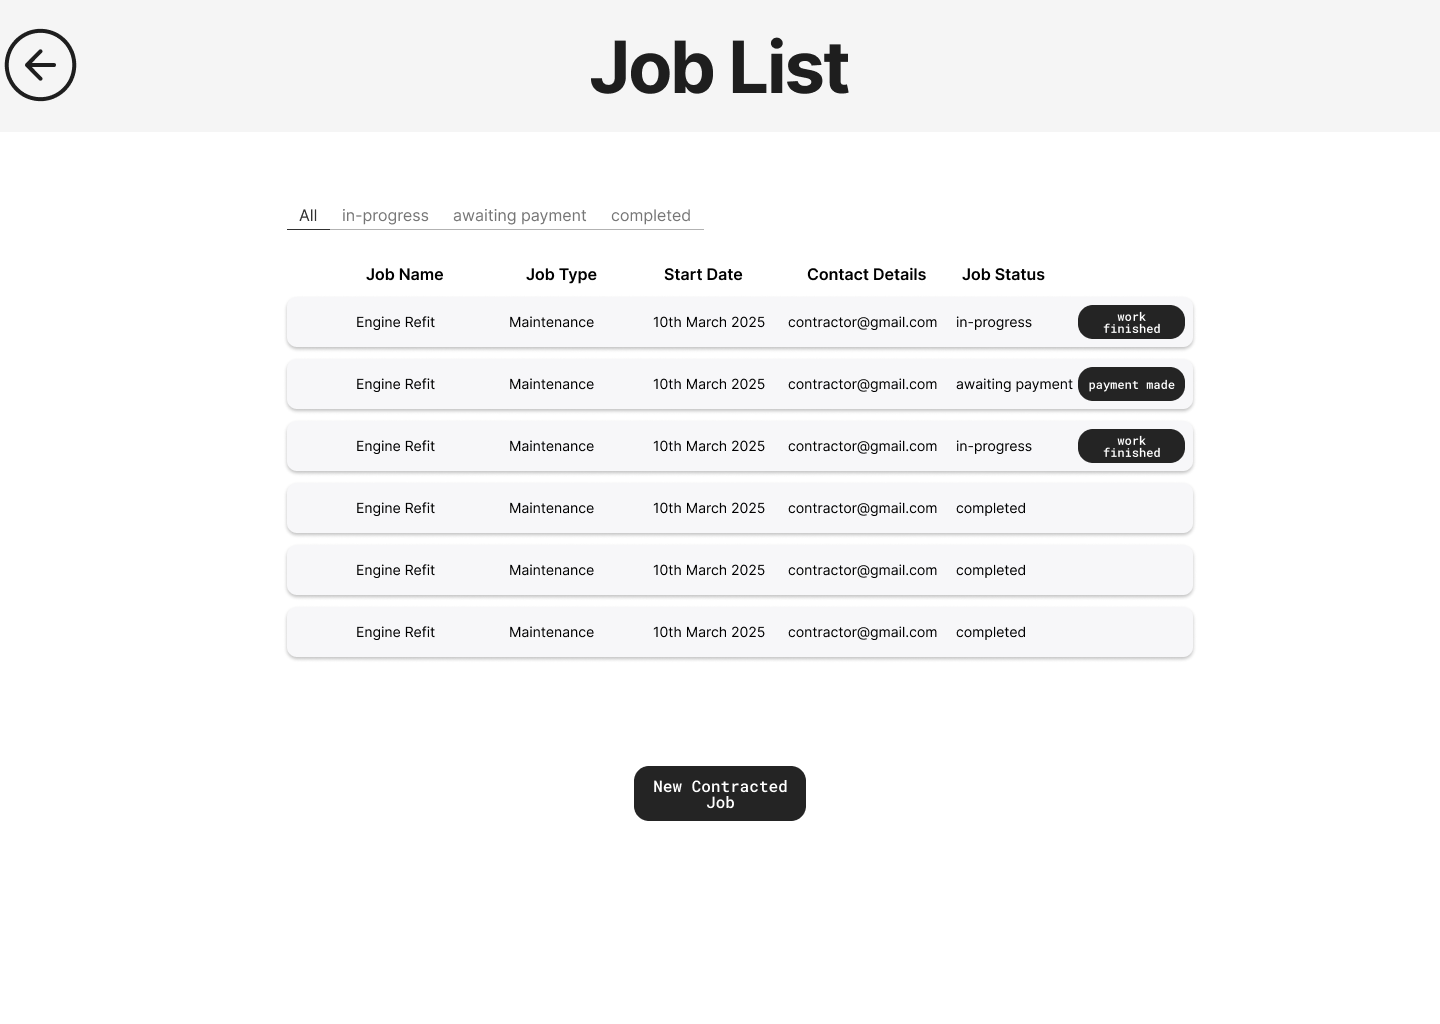
\includegraphics[width=0.75\linewidth]{../mockup-screens/Contractor-mockups/job list.png}
        \caption{Create menu}
        \label{fig:contractor-assignment-form}
    \end{figure}	

    \begin{figure}[H]
        \centering
        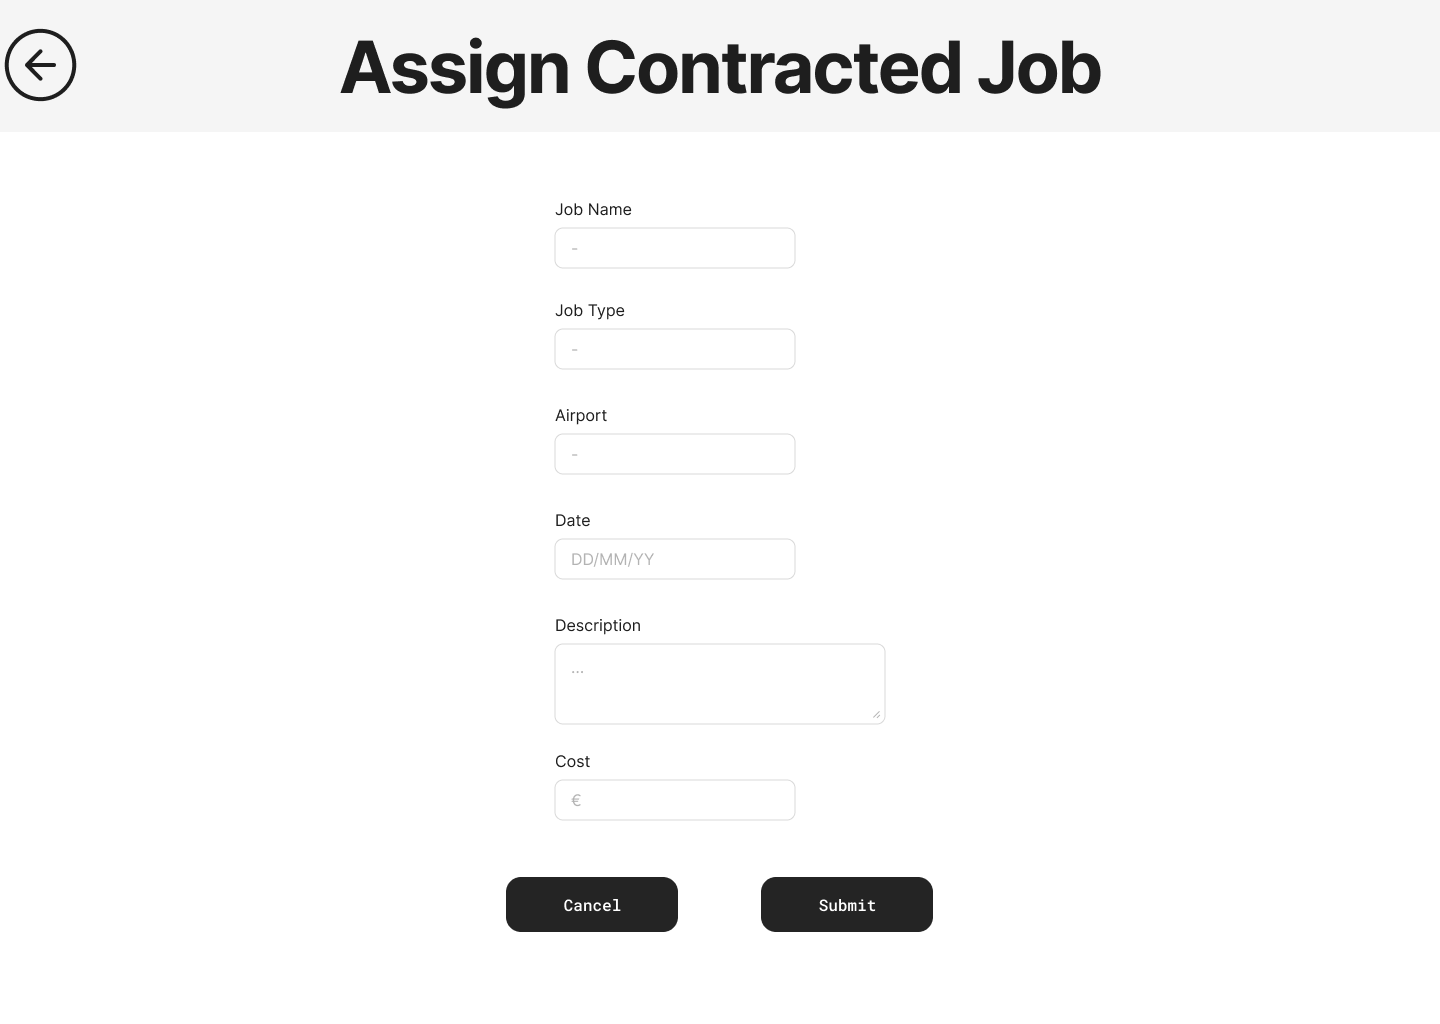
\includegraphics[width=0.75\linewidth]{../mockup-screens/Contractor-mockups/assign contracted job.png}
        \caption{Create menu}
        \label{fig:contractor-one-time-adjustment}
    \end{figure}	

	
	\section{Οφέλη του Συστήματος}
	\begin{enumerate}
		\item Αποδοτικότητα: Οι βελτιστοποιημένες διαδρομές και η κατανομή πόρων μειώνουν το λειτουργικό κόστος και βελτιώνουν την αποδοτικότητα.
		\item Ακρίβεια: Οι αυτοματοποιημένοι υπολογισμοί και αναφορές διασφαλίζουν την ακριβή ανάλυση δεδομένων.
		\item Ευελιξία: Το σύστημα μπορεί να προσαρμοστεί σε διαφορετικά μεγέθη αεροπορικών εταιρειών και επιχειρησιακές ανάγκες.
		\item Φιλικό προς το χρήστη: Ένα ασφαλές σύστημα σύνδεσης και έλεγχος πρόσβασης βάσει ρόλων καθιστούν το σύστημα εύκολο στη χρήση για όλους τους υπαλλήλους.
	\end{enumerate}
	
	\subsection{Περιφερειακά και Συσκευές}
	Η εφαρομγή έχει πολύ χαμηλές απαιτήσεις. Χρειάζεται μόνο:
	\begin{enumerate}
		\item υπολογιστή που έχει εγκατεστημένο το java 
		\item πληκτρολόγιο και ποντίκη
	\end{enumerate}
	Είναι απαραίτητο να έχουμε τις λιγότερες απαιτήσεις που γίνεται γιατί η εταιρία δεν θα θέλει
	να ξοδεύει άσκοπα λεφτά σε ακριβά υπολογιστικά συστήματα όταν θα μπορούν να κάνουν την ίδια
	δουλεία σε πιο φτηνούς υπολογιστές. Συχνά οι υπολογιστές που διαθέτουν αεροπορικές εταιρίες
	είναι πολύ παλίες και έχουν πολύ παλιά λογισμικά.
	
	\section{Stakeholders}
	Αυτή η εφαρομγή είναι πάρα πολύ σημαντική για οποιαδήποτε αεροπορική εταιρία για να μπορεί να οργανώσει τους
	πόρους που έχει. Το κάνει πολύ εύκολο για τους διαχειριστές της εταιρίες να μπορούν να δουν ανά πάσα στιγμή
	πράγματα όπως της πτήσης, αεροπλάνα και προσωπικό και πολλά άλλα...

	Αυτό είναι πολύ χρήσιμο για τους διαχειριστές γιατί ξοδεύει χρόνο καθώς όλη η πληροφορία είναι στο ίδιο μέρος
	και δεν χρειάζεται να ρωτάει τα άτομα της εταιρίας για πληροφορίες όπως τον αριθμό των αεροπλάνων που έχουν
	ακινοτοποιηθεί για επισκευές. Επίσης τους δίνει την δυνατότητα να αποφεύγει λάθη στο χρονοπρογραμματισμό
	πτήσεων καθώς το σύστημα εντοπίζει αν ένας αεροσυνοδός δεν θα μπορεί να είναι σε μια πτήση μια συγκεκριμμένη στιγμή.

	Το σύστημα αυτό επίσης θα χρησιμοποιείται από πιλότους για να ανεβάζουν αναφορές για την κατάσταση του αεροπλάνου.
	Αυτό σημαίνει ότι θα μπορούμε να καταγράφουμε όλο το ιστορικό του αεροπλάνου που μπορεί να βοηθήσει τον μηχανικό
	που κάνει επισκευές να εντωπίζει πιο γρήγορα τα προβλήματα του αεροπλάνου και πιθανός να εντωπίσει προβλήματα πριν
	γίνουν επικίνδυνα. Επίσης ο πιλότος μπορεί να ακινητοποιήσει το αεροπλάνο μέχρι να γίνουν επισκευές που βοηθάει
	το προσωπικό που φτιάχνει τα δρομολόγια για να μπορούν γρήγορα να ακυρώσουν τις μελλοντικές πτήσεις και να αλλάξουν
	το πρόγραμμα ανάλογα των άλλων αεροπλάνων. 

	Επίσης βοηθάει το προσωπικό που κλείνει εισητήρια για επιβάτες για να κάνουν την δουλειά τους πιο γρήγορα και βοηθάει
	τον πελάτη καθώς του δίνει ηλεκρονική επιβεβαίωση για τα στοιχεία της πτήσης.
	
	\section{Συμπέρασμα}
	Το SkyOps είναι ένα ισχυρό εργαλείο για τις 
	αεροπορικές εταιρείες που επιθυμούν να βελτιστοποιήσουν τις 
	δραστηριότητές τους, να μειώσουν το κόστος και να βελτιώσουν 
	την ποιότητα των υπηρεσιών. Αυτοματοποιώντας πολύπλοκες 
	διαδικασίες και παρέχοντας λεπτομερείς πληροφορίες, το σύστημα 
	βοηθά τις αεροπορικές εταιρείες να παραμείνουν ανταγωνιστικές 
	σε έναν κλάδο με γρήγορους ρυθμούς.
	
\end{document}
